\section{金剛般若波羅蜜經}
六祖以前,禪宗以《楞伽》印心,此後《金剛經》即代替了《楞伽》。宋代,出家人的考試,有《金剛經》一科,可見他的弘通之盛!
\paragraph{中國佛教的特點}
一重實行:如臺、賢、禪、淨各宗,都注重行持,尤重於從定發慧的體悟。二好簡易,國人的習性好簡,卷帙浩繁的經論,是極難普遍流通的。

\begin{quote}
  「修多羅次第所顯」
\end{quote}

\begin{quote}
  無著說:「金剛難壞句義聚,一切聖人不能入」。
\end{quote}

\begin{quote}
  世親說:「法門句義及次第,世間不解離明慧」。
\end{quote}

\subsection{经题}
\subsubsection{金刚} 堅常 明淨 快利
\subsubsection{般若} 慧 \footnote{須菩提在般若會上,曾提出四個問題——何者般若,何名般若,般若何用,般若屬誰}
\begin{enumerate}
  \item 實相般若 離一切相——言語相、文字相、心緣相,而無可取著的。
    \footnote{《智論》說:「般若波羅蜜者,即一切諸法實相,不可破,不可壞」}
    \footnote{《智論》說:「般若如大火聚,四邊不可觸」}
    \footnote{古德說:「說似一物即不中」}
    \footnote{《法華經》說:「唯佛與佛乃能究盡諸法實相,所謂:諸法如是相,如是性,如是體,如是力,如是作,如是因,如是緣,如是果,如是報,如是本末究竟等」}
    \footnote{《中論》說:「空則不可說,非空不可說,共不共叵說,但以假名說」}
    \footnote{「不壞假名而說法性」}
    \footnote{《中論》說:「一切實非實,亦實亦非實,非實非非實,是名諸佛法」}
    \footnote{「凡所有相,皆是虛妄;若見諸相非相,則見如來」}
  \item 觀照般若
    \footnote{《智論》說:「從初發心求一切種智,於其中間,知諸法實相慧,是般若波羅蜜」}
    \footnote{二乘行者得無我我所慧,解脫生死,可以稱為般若;但也不是《般若經》所說的般若。大乘的諸法實相慧,要有大悲方便助成的}
    \footnote{《智論》說:「般若是一法,隨機而異稱」}
    \footnote{《智論》說:「未成就名空,已成就名般若」}
    \footnote{「因名般若,果名薩婆若」}
    \footnote{《智論》這樣說:「般若將入畢竟空,絕諸戲論;方便將出畢竟空,嚴土熟生」。}
  \item 文字般若 \footnote{「般若當於何求?當於須菩提所說中求」}
\end{enumerate}
\paragraph{初學般若,應先於文教聽聞、受持,以聞思慧為主。}
經合理的思考、明達,進而攝心以觀察緣起無自性,即觀照般若,以思修慧為主。如得離一切妄想戲論,現覺實相,即實相般若了。這三者,同明般若而各有所重,如意在實相,即能 所並寂而非名言思惟可及。如意在觀慧,即依境成觀,以離相無住的相應為宗。如意在文字,即重在安立二諦,抉擇空有。
\footnote{如求水,拙慧者非鑿開冰層,從冰下去求水不可;而巧慧者知道冰即是水,一經般若烈火,冰都是水了}
\begin{quote}
  「離三解脫門,無道無果」
\end{quote}
\subsubsection{波羅蜜}
梵語波羅蜜,譯為到彼岸,簡譯為度。
\subsubsection{經}
梵語修多羅,譯為經

\begin{enumerate}
  \item 玄奘等傳說 般若是能斷的智慧,金剛如所斷的煩惱。
  \item 羅什下的傳說 金剛比喻般若
\end{enumerate}

\subsection{五種菩提}
\begin{enumerate}
  \item 發心菩提:凡夫於生死中,初發上求佛道、下化眾生的大心,名發阿耨多羅三藐三菩提心,所以名為發心菩提。
  \item 伏心菩提:發心以後,就依本願去修行,從六度的實行中,漸漸降伏煩惱,漸與性空相應,所以名為伏心菩提。
    \footnote{七地以前}
  \item 明心菩提:折伏粗煩惱後,進而切實修習止觀,斷一切煩惱,徹證離相菩提——實相,所以名為明心菩提。
    \footnote{望前般若道說,是證悟;望後方便道說,是發心。前發心菩提,是發世俗菩提心;而明心菩提是發勝義菩提心。悟到一切法本清淨,本來涅槃,名得真菩提心}
  \item 出到菩提:發勝義菩提心,得無生忍,以後即修方便道,莊嚴佛國,成熟眾生;漸漸的出離三界,到達究竟佛果,所以名為出到菩提。
  \item 究竟菩提:斷煩惱習氣究竟,自利利他究竟,即圓滿證得究竟的無上正等菩提。
\end{enumerate}
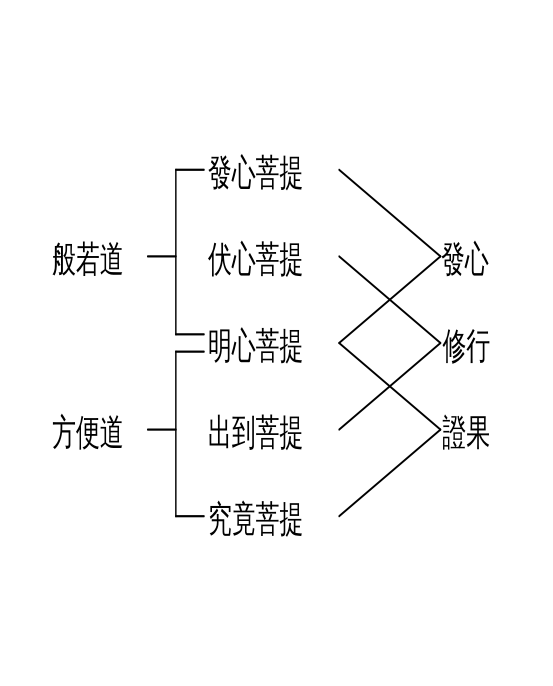
\includegraphics[scale=0.5]{释家/images/五種菩提.png}

\subsection{版本}
本經,什公第一次譯出。除這,還有五種譯本,就是:元魏菩提留支的第二譯,陳真諦的第三譯,隋達摩笈多的第四譯,唐玄奘的第五譯,唐義淨的第六譯。在六譯中通常流通的,即是什公的初譯。其後的五譯,實是同一法相學系的誦本;如菩提留支譯,達摩笈多譯等,都是依無著、世親的釋本而譯出。唯有什公 所譯,是中觀家的誦本,所以彼此間,每有不同之處。要知道印度原本,即有多少出入;如玄奘譯本也有與無著、世親所依本不同處。

\subsection{正文}
\paragraph{信为能入}
無信如無手,不能探取佛法寶藏;無智如無目,不能明達佛法深義。
\paragraph{千二百五十人}
佛在鹿苑,初度憍陳如等五比丘;接著又有耶舍等五十多人,隨佛出家;三迦葉率領他的徒眾,從佛出家,就有一千多眾了;王舍城的舍利弗、目犍連,又帶了二百五十弟子來出家;於是佛的初期出家弟子,就有千二百五十人了。
\paragraph{比丘}
譯為乞士,就是「外乞食以養色身,內乞法以資慧命」

\subsubsection{衣}
\begin{enumerate}
  \item 五衣名安荼會,不論睡覺做事,就是大小便,也不離身,這是內衣。
  \item 七衣名鬱多羅僧,即入眾的常禮服,在大眾中所穿。
  \item 大衣名僧伽黎,即複衣,在乞食、說法等時所穿的,是佛教大禮服。
\end{enumerate}

\paragraph{護念} 即攝受,對於久學而已入正定聚的 菩薩,佛能善巧的攝受他,使他契入甚深的佛道,得如來護念的究竟利益。
\paragraph{付囑} 即叮嚀教誡,對於初學而未入正定聚的菩薩,佛能善巧教導,使他不捨大乘行,能勇猛的進修。

\begin{quote}
  「菩薩但從大悲心生,不從餘善生」;「為利眾生而成佛」
\end{quote}

\begin{quote}
  阿耨多羅\footnote{無上}三藐\footnote{遍正}三菩提\footnote{覺}
\end{quote}

\subsubsection{涅磐}
\paragraph{有餘(依)涅槃}
通達一切法的寂滅性,離煩惱而得到內心的解脫,即是涅槃。但由前生惑業所感的果報身還在,從身體而來的痛苦,還未能解除。
\paragraph{無餘(依)涅槃}
無學捨身而入無量無數的法性, 不再有物我、自他、身心的拘礙,名為無餘。
\footnote{菩薩安住無住大涅槃,即此無餘涅槃的無方大用,能悲願無盡,不證實際罷了}

\subsubsection{悲}
菩提心是即空的菩提心,與菩提心相應的悲願,即無緣大悲。
見到眾生的痛苦,生起濟拔的惻隱心,以世間的財法去救濟他,是眾生緣悲。
如見眾生為相續、和合的假我,法生苦生,法滅苦滅,因而起悲濟心,是法緣悲。
如能觀諸法從緣,都無真實的自性,悟入法性空,緣即空而緣起的假我,生大悲心,願度如幻眾生,這是無緣大悲。

\begin{quote}
《般若經》說:「一切智智相應作意(即菩提心),大悲為上首,無所得——即般若空慧為方便」。\footnote{悲心不具足而慧力強,要退墮聲聞乘的。慧力不足而悲心強,要流於世俗而成所謂「敗壞菩薩」的。}
\end{quote}


\begin{quote}
  「見緣起即見法,見法即見佛」
\end{quote}

\begin{quote}
  實信,在聲聞法中,即證須陀洹,得四不壞信——四證淨;大乘在見道淨 心地。
  \footnote{由信順而信忍,由信忍而達到信智一如的證信。}
\end{quote}

\begin{quote}
  「一切法不信則信般若,一切法不生則般若生」
\end{quote}

\begin{quote}
  「聽聞正法,如理作意,法隨法行」
\end{quote}

\subsubsection{微尘}
\paragraph{声闻}
主張色法——物質有極微細的塵粒,即是不可再分析的個體;無論如何分析,終究有這最後的質素
\paragraph{中观}
一切法是因緣和合生的,緣生的諸法中,雖有顯現為色法的形態,而且是有粗有細的。不論為粗的細的,都是 無常、無我而自性空寂的。
\paragraph{唯识}
是心識變現的,是由內心的色種子,變現這似乎外在的色法,而實不是離心有自相的。

\subsubsection{忍}
\begin{enumerate}
  \item 忍受人事間的苦迫,叫生忍\footnote{佛法勸人忍辱,是勸人學菩薩,是無我大悲的實踐,非奴隸式的忍辱!}
  \item 忍受身心的勞苦病苦,以及風雨寒熱等苦,叫法忍
  \item 忍可諸法無生性,叫無生忍\footnote{無生忍即般若慧}
\end{enumerate}
